\documentclass[a4paper]{article}

% Includes packages relevant to Senior Lab

% character set specifications
\usepackage[english]{babel}
\usepackage[utf8]{inputenc}

% increased vertical spacing for tables
\newcommand\topVspace{\rule{0pt}{2.6ex}}      
\newcommand\bottomVspace{\rule[-1.2ex]{0pt}{0pt}} 

% extra unicode characters
\DeclareUnicodeCharacter{3BC}{\(\mu\)}
\DeclareUnicodeCharacter{3C1}{\(\rho\)}
\DeclareUnicodeCharacter{2080}{\(_0\)}
\DeclareUnicodeCharacter{2081}{\(_1\)}
\DeclareUnicodeCharacter{2082}{\(_2\)}
\DeclareUnicodeCharacter{3B5}{\(\epsilon\)}
\DeclareUnicodeCharacter{3B1}{\(\alpha\)}

% SI Units
\usepackage{siunitx}

% extra SI units
\DeclareSIUnit\gauss{G}

% enable scientific notation
\sisetup{scientific-notation = engineering, exponent-to-prefix}

% draw pretty lines
\usepackage{tikz}
\usetikzlibrary{datavisualization}
\usepackage{circuitikz}

% manual tabbing
\setlength{\parindent}{0pt}
\def\qq{\qquad}

% include graphics
\usepackage{graphicx}

% increased control over figure placement
\usepackage{float}

% box answers
\usepackage{tcolorbox}

% enable multiple section levels
\usepackage{titlesec}

% define `\subsubsubsection` command
\titleclass{\subsubsubsection}{straight}[\subsection]
\newcounter{subsubsubsection}[subsubsection]
\renewcommand\thesubsubsubsection{\thesubsubsection.\arabic{subsubsubsection}}
\titleformat{\subsubsubsection}
        {\normalfont\normalsize\bfseries}{\thesubsubsubsection}{1em}{}
\titlespacing*{\subsubsubsection}
{0pt}{3.25ex plus 1ex minus .2ex}{1.5ex plus .2ex}
\setcounter{secnumdepth}{4}

% get align environment (among other things)
\usepackage{amsmath}

% bold in math mode
\usepackage{bm}

% get \mathbb (among other things)
\usepackage{amssymb}

\usepackage{array}

% plotting
\usepackage{pgfplots}

% enable external references
\usepackage{hyperref}

% include code
\usepackage[cache=false]{minted}
\setminted{linenos, frame=lines, texcomments}

% adjust margins of individual pages (for shoving figures into place)
\usepackage{changepage}

% rotate figures
\usepackage{rotating}


\usepackage{caption}
\renewcommand{\thetable}{\arabic{section}.\arabic{table}}

\title{PHY 4210-01 Senior Lab \\Lab P-5: Hall Effect in Semiconductors}

\author{Sarah Arends \\
        Jacquelyne Miksanek \\
        Ryan Wojtyla \\ \\
        Instructor: Jerry Collins II}

\date{February 21, 2019}
\begin{document}
\maketitle

\begin{abstract}
%physics of experiment
%apparatus used
%what was measured
%Results
\qq The Hall Effect was investigated through a series of experiments
using p-type, n-type, and pure Germanium, as well as pure
Zinc. Experiments involved measurements and manipulation of the Hall
voltage, sample voltage, current, magnetic field strength, and
temperature. Temperature and current were monitored with the
semiconductor mount, and field strength was measured using a Hall
effect probe. Several parameters of the semiconductor materials were
calculated, including the Hall constant and density of charge
carriers. Because there were about 12 different experiments conducted,
the results will not all be restated here. Instead, please refer to the
conclusion of each respective task.
\end{abstract}

\newpage

\setcounter{tocdepth}{2}
\tableofcontents

\newpage

\section{Theory of the Experiment}
%A short presentation of the concepts and formulas related to the experiment.

\qq When an electric current flows through a conductor inside of a
magnetic field, that field exerts a force on the charge carriers as
they move. This force is the Lorentz force. The Lorentz force causes
the charge carriers to accumulate on one side of the conductor, which
will then balance the magnetic influence from the field and produce a
voltage that can be measured across the conductor. This describes the
Hall effect. The Hall voltage can be measured by a Hall probe that is
placed in the magnetic field. Please note that the Hall effect is
different for differing charge carriers, as the polarity of the Hall
voltage differs for negative and positive charge carriers.

\subsection{Deriving the Hall Voltage Equation}

\begin{align*}
V_(Hall) = \frac{I*B}{n*e*t}
\end{align*}
\qq  Please note that 'I' is the current through the sample, 'B' is the
 applied magnetic field, 'n' is the charge carrier concentration, 'e'
 is the elementary charge, and 't' is the sample thickness.

\begin{align*}
F_B = q*v*B
F_E = E*q = \Big(\frac{V_H}{d}\Big)*q
F_B = F_E
q*v*B = \Big(\frac{V_H}{d}\Big)*q
v*B = \frac{v_H}{d}
v_H = B*v*d
v = \frac{I}{n*e*A}
v_H = \frac{B*I*d}{n*e*A}
A = t*d
v_H = \frac{B*I*d}{n*e*t*d}
v_H = \frac{I*B}{n*e*t}
\end{align*}

\section{Hall Effect in P-Germanium}

\subsection{Task 1}

\qq The Hall voltage's dependence on the current through the sample
was determined while holding the magnetic field and temperature
constant. Please note that the manual called for the magnetic field to
be held at 250 mT, but this corresponds to a current that exceeds the
maximum allowed by the coils. The field was instead kept at 144 mT,
which corresponds to a current of 4A.

\subsubsection{Data Analysis and Results}
%Graphs, figures, and tables with captions
%Results with error analysis
%Calculate discrepancies from theory
%Discuss results and uncertainties

% Discuss results
\qq There is a linear relationship between the Hall Voltage and the sample 
current, which is shown by the following equation, where $\alpha$ is
the proportionality constant:
\begin{align*}
U_H = \alpha * I
\end{align*}
The data was plotted in figure \ref{task21plot}. Through the use of
linear regression, the proportionality constant was determined to be
$0.943 \pm \num{5.54e-3}$ V/A.

% Experimental data 
\begin{figure}[H]
\centering
% uncomment the line below to add image
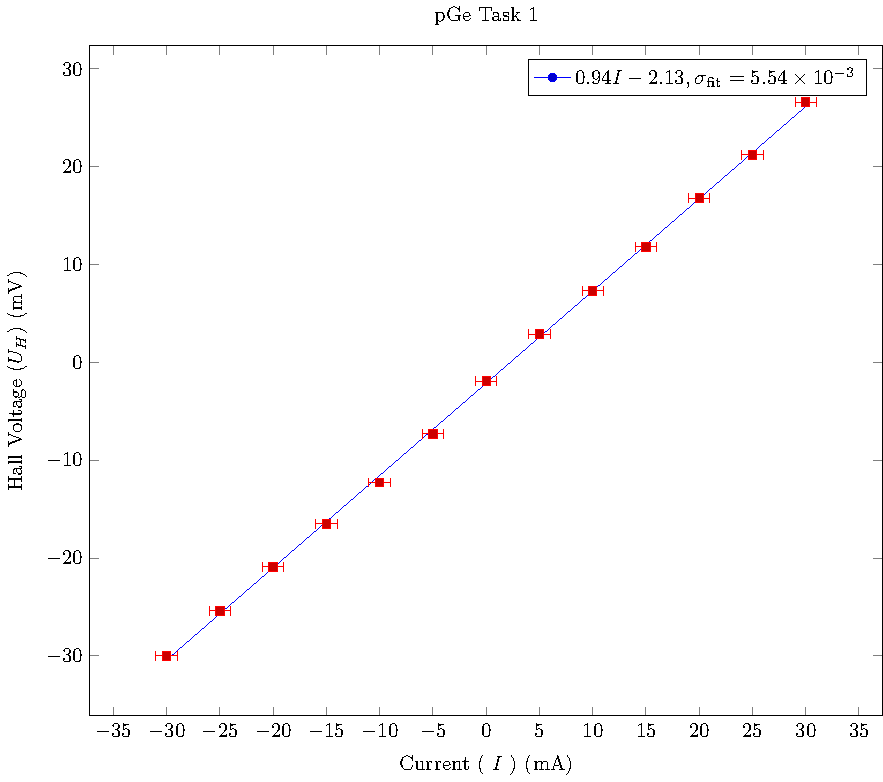
\includegraphics[width=0.7\textwidth]{PGePlots/Task1/pGeTask1.pdf}
\captionof{figure}{Hall voltage as a function of sample current 
in p-type Germanium. The linear fit has an $R^2$ value of 1.}
\label{task21plot}
\end{figure}

% Calculate theoretical proportionality constant
\qq From the equation defining the Hall Voltage, one can derive an
expression for $V_{Hall}/I$, which represents the slope or
proportionality constant $\alpha$. The expression is used to obtain a
value for $\alpha_{theo}$ below, where $B$ is the applied magnetic
field, $n$ is the density of charge carriers, $e$ is the elementary
charge, and $t$ is the sample thickness.
\begin{align*}
\alpha_{theo} &= \frac{B}{net} \\
              &= \frac{0.144}{(1.5 * 10^(21))*(1.6 * 10^(-19))*(1.0 * 10^(-3))}
			  &= 0.6 \\
\end{align*}

\subsubsection{Conclusion}
%Brief summary, discussion of results and theory
The experimental constant of proportionality $\alpha = 0.943 $ V/A is
within 54 $\sigma$ of the theoretical value $\alpha_{theo} =
0.6$ V/A. This discrepancy in the face of such a well fitting line is a sign of
systematic rather than random error. Sources of systematic error include energy
escaping the system or an offset in the power supply.

\subsection{Task 2}

\qq The sample voltage as a function of the positive magnetic field
induction was determined. The control current was held at a constant
30 mA. The resistance was computed from the sample voltage, and
expressed as a change in resistance relative to the resistance with no
field.

\subsubsection{Data Analysis and Results}
%Graphs, figures, and tables with captions
%Results with error analysis
%Calculate discrepancies from theory
%Discuss results and uncertainties
\qq Instead of directly plotting the resistance against the field
strength. A "normalized difference" was computed by dividing the total
change in resistance by the resistance with no applied field,
i.e. $\frac{R_m - R_0}{R_0}$, where $R_m$ represents the measured
resistance and $R_0$ represent the resistance at $B=0$. The change in
resistance associated with a changing magnetic field implies a change
in the mean free path of the charge carriers (holes). The resultant
graph in figure \ref{task22plot} shows a quadratic change in this
expression as a function of the increasing induced magnetic field
strength, which is the expected relationship between the given
quantities.

% Experimental data 
\begin{figure}[H]
\centering
% uncomment the line below to add image
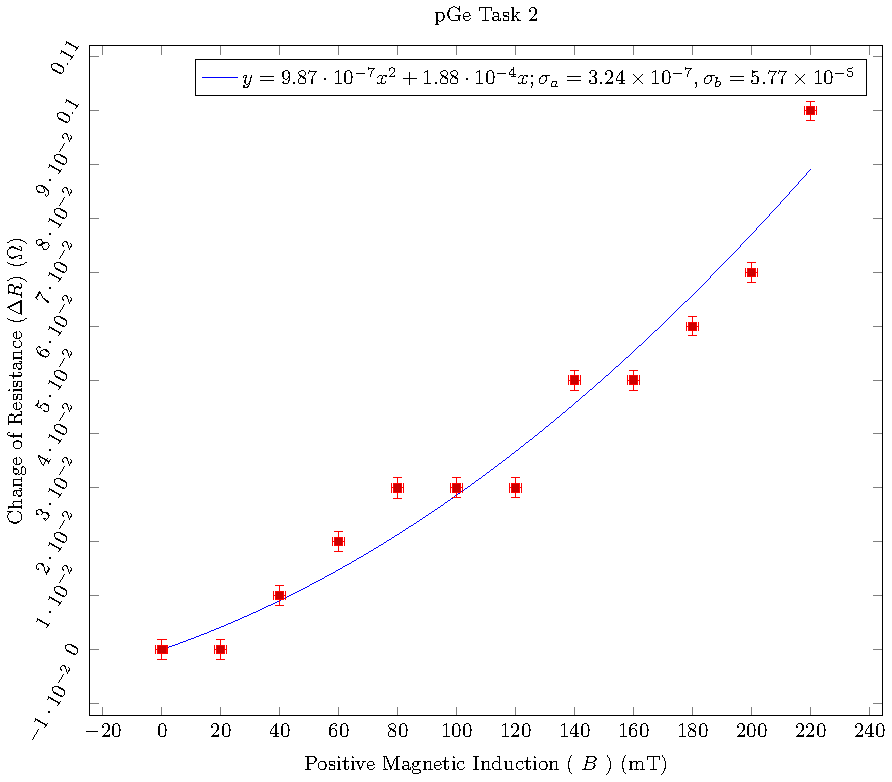
\includegraphics[width=0.7\textwidth]{PGePlots/Task2/pGeTask2.pdf}
\captionof{figure}{Normalized change in resistance against applied
  field strength. The determined $R^2$ value was 0.969}
\label{task22plot}
\end{figure}

\subsubsection{Conclusion}
%Brief summary, discussion of results and theory
\qq The functional relationship between normalized change in resistance
and the applied magnetic field strength was quadratic, as expected.

\subsection{Task 3}

\qq A constant current of 30 mA is applied, and the sample voltage is
measured as a function of temperature. The magnetic field remains off
for this task. The manual states that the maximum applied temperature
is $140^o$ C. In order to avoid damaging the sample, the temperature
was instead limited to $110^o$ C. Note that the sample was heated to
this maximum temperature, and then the sample voltage was taken as the
temperature cooled.

\subsubsection{Data Analysis and Results}
%Graphs, figures, and tables with captions
%Results with error analysis
%Calculate discrepancies from theory
%Discuss results and uncertainties
\qq Sample voltage and temperature were measured, with no external
field applied. The reciprocal of the voltage was plotted against the
reciprocal of the temperature. The data, shown in figure
\ref{task23plot}, can be represented by a quadratic function, with a
minimum occurring around 3 $K^{-1}$.

% Experimental data 
\begin{figure}[H]
\centering
% uncomment the line below to add image
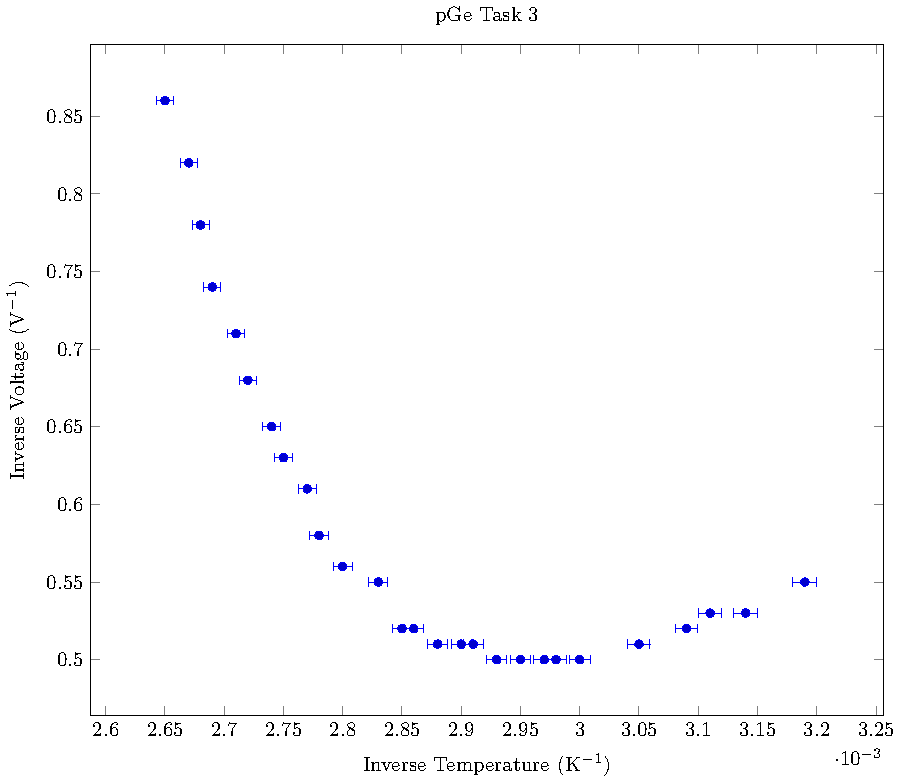
\includegraphics[width=0.7\textwidth]{PGePlots/Task3/pGeTask3Tot.pdf}
\captionof{figure}{Inverse voltage is plotted against inverse temperature.}
\label{task23plot}
\end{figure}

\qq In order to obtain meaningful information from the data in figure
\ref{task23plot}, one can manipulate the data to uncover a linear
relationship. The intrinsic conductivity can be approximated as the
inverse voltage, since the temperature is constant. Conductivity is
related to inverse temperature by the following function:
$$\sigma = \sigma_0 e^{-E_g/2kT}$$

% Calculated data 
\begin{figure}[H]
\centering
% uncomment the line below to add image
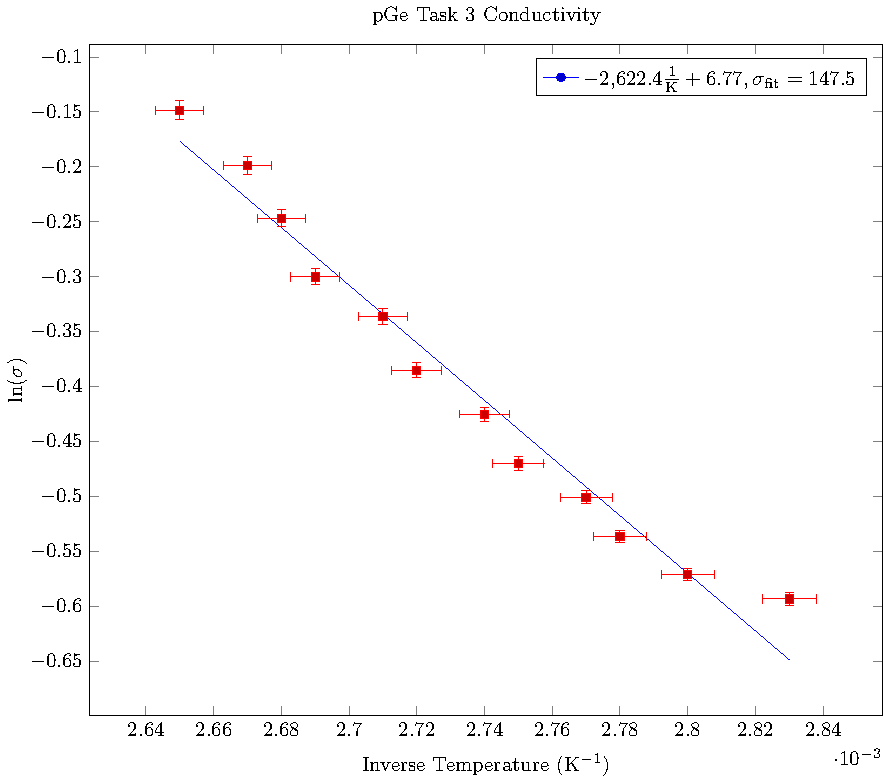
\includegraphics[width=0.7\textwidth]{PGePlots/Task3/pGeTask3Ln.pdf}
\captionof{figure}{Natural logarithm of conductivity versus inverse temperature}
\label{task23plotLINEAR}
\end{figure}

\qq If the natural logarithm of conductivity is plotted against
inverse temperature, as shown in figure \ref{task23plotLINEAR}, it
will obey a linear relationship with slope equal to $-
\frac{E_g}{2k}$. Linear regression yields a slope of $-2622 \pm
147.5$ K. Recalling that $k$ is Boltzmann's constant, we
compute the band gap energy as follows.

% Compute Eg experimentally
\begin{align*}
E_g &= - \text{slope} \times 2k \\
    &= - (-2622 \; K) \times 2 
       \Big( 8.63 \times 10^{-5} \frac{eV}{K} \Big) \\
    &= 0.45 eV \\
\end{align*}

% Experimental error
The associated error in $E_{g_{exp}}$ can be computed from the error in the slope.
\begin{align*}
  \delta_{Eg_{exp}} &= 2 k \sigma\\
  \delta_{Eg_{exp}} &= 2 (\SI{8.63e-5}{\electronvolt\per\kelvin}) (\SI{148}{\kelvin}) \\
  \delta_{Eg_{exp}} &= \SI{0.0255}{\electronvolt}
\end{align*}

% Difference and discrepancy
\qq The discrepancy is computed between the experimental value of
$E_g$ and the theoretical value $E_{g_{theo}} = 0.72$ eV. The
associated error in the discrepancy will be taken as the error in the
experimental value, since the theoretical value has no associated
error.
\begin{align*}
\delta_{E_g} &= | E_{g_{exp}} - E_{g_{theo}} | \\
		     &= | 0.49 - 0.72 | \\
		     &= 0.23 eV \\
\end{align*}

\subsubsection{Conclusion}
%Brief summary, discussion of results and theory
\qq The experimental energy gap $E_{g_{exp}} = 0.49 eV$ is within
\num{0.00182} $\sigma$ of the theoretical value $E_{g_{theo}} = 0.72 eV$,
thus the values are in agreement.

\subsection{Task 4}

\qq The Hall voltage was measured as a function of the magnetic
induction. This time the temperature is held constant at room
temperature, and the current is held constant at 30 mA. The manual
states that the applied magnetic field should reach 300 mT,
however, the strength was limited to 290 mT. This was done in
order to avoid applying excessive current and overheating the coils. 
Note that the highest current applied to the coils was 5.98
Amperes.

\subsubsection{Data Analysis and Results}
%Graphs, figures, and tables with captions
%Results with error analysis
%Calculate discrepancies from theory
%Discuss results and uncertainties
\qq The Hall voltage was plotted against the magnetic field strength
with both positive and negative polarities. The resultant graph, shown
in figure \ref{task24plot}, was given a linear fit, with an $R^2$
value of 0.999.

% Calculated data 
\begin{figure}[H]
\centering
% uncomment the line below to add image
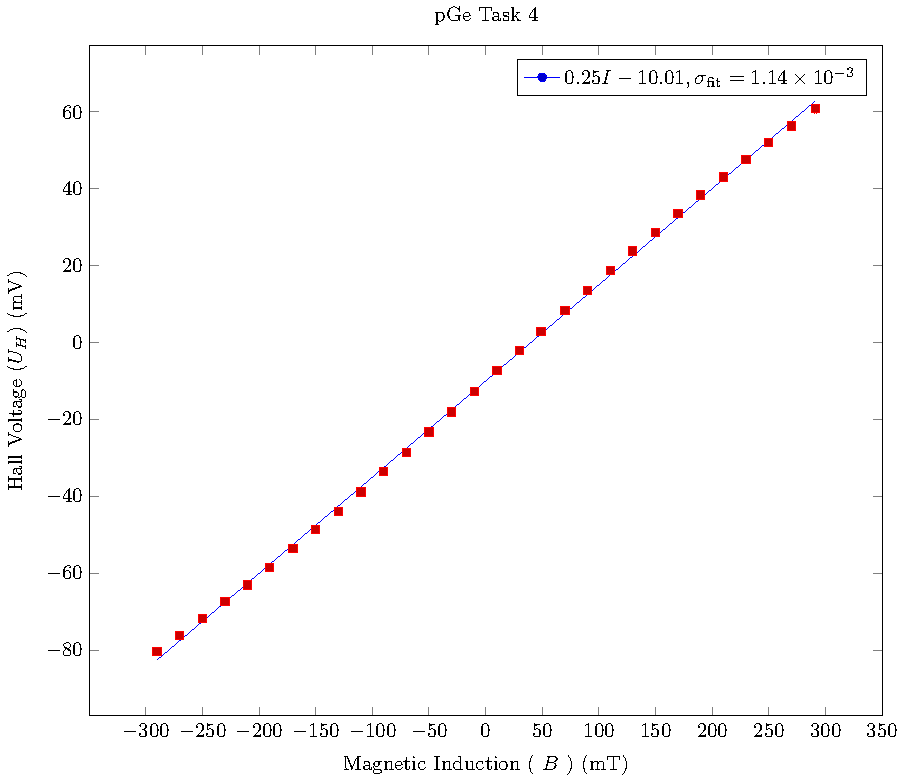
\includegraphics[width=0.7\textwidth]{PGePlots/Task4/pGeTask4.pdf}
\captionof{figure}{Hall voltage plotted as a function of applied
  magnetic field strength.}
\label{task24plot}
\end{figure}

% Experimental calculation of hall constant
\qq The experimental Hall constant is the slope, \( b =
\SI{0.25}{\volt\per\tesla} \), of Figure (\ref{task24plot})
multiplied by \( \frac{d}{I} \), where \( d = \SI{1e-3}{\meter} \) is the
thickness of the sample and \( I = \SI{30}{\milli\ampere} \) is the applied
current. 

\begin{align*}
  R_{\text{H}} &= b \frac{d}{I} \\
  R_{\text{H}} &= (0.25) \frac{(\num{1e-3})}{(\num{30e-3})} \\
  R_{\text{H}} &= \num{0.00833}\si{\cubic\meter\per\ampere\per\second} \\
\end{align*}

% Error in experimental hall constant
\qq Since the only variable, the slope \( b \), is begin multiplied by the constant
\( \frac{d}{I} = \num{0.0333} \), the error in the experimental hall constant is
merely the error in the slope, \( \delta b = \SI{1.14e-3}{\volt\per\tesla} \),
multiplied by the constant.

\begin{align*}
  \delta R_{\text{H}} &= \delta b \frac{d}{I} \\
  \delta R_{\text{H}} &= (\num{1.14e-3}) (\num{0.0333}) \\
  \delta R_{\text{H}} &= \SI{3.80e-5}{\cubic\meter\per\ampere\per\second} \\
\end{align*}

% Discrepancy compared to theory
\qq The theoretical value of the Hall constant is
\SI{4.17e-3}{\cubic\meter\per\ampere\per\second}. Therefore, the discrepancy
between our experimental value and this theoretical value is

\begin{align*}
  \Delta_{R_{\text{H}}} &= | R_{\text{H}_{\text{theo}}} - R_{\text{H}_{\text{exp}}} | \\
  \Delta_{R_{\text{H}}} &= | (\num{4.17e-3}) - (\num{8.33e-3}) | \\
  \Delta_{R_{\text{H}}} &= \SI{4.16e-3}{\cubic\meter\per\ampere\per\second} \\
\end{align*}

% Experimental calculation of carrier concentration
\qq The carrier concentration is found with \( p =
\frac{1}{\si{\elementarycharge} R_{\text{H}}} \), where \(
\si{\elementarycharge} = \SI{1.60e-19}{\coulomb} \) is the elementary charge and
\( R_{\text{H}} \) is either the theoretical or experimental value of the Hall constant.
The experimental value of the carrier concentration is determined by using the
experimental for the Hall constant.

\begin{align*}
  p_{\text{exp}} &= \frac{1}{\si{\elementarycharge} R_{\text{H}_{\text{exp}}}}
  \\
  p_{\text{exp}} &= \frac{1}{(\SI{1.60e-19}{\coulomb})
      (\SI{8.33e-3}{\cubic\meter\per\ampere\per\second})} \\
  p_{\text{exp}} &= \SI{7.50e20}{\per\cubic\meter} \\
\end{align*}

The error in the experimental value of the carrier concentration is determined
with \( \delta p_{\text{exp}} = | p_{\text{exp}} | \frac{\delta
  R_{\text{H}_{\text{exp}}}}{R_{\text{H}_{\text{exp}}}} \)

% Theoretical carrier concentration
\qq The theoretical carrier concentration, \( p_{\text{theo}} \), is determined in a
similar manner; the theoretical value of the Hall constant is used rather than
the experimental one.

\begin{align*}
  p_{\text{theo}} &= \frac{1}{\si{\elementarycharge} R_{\text{H}_{\text{theo}}}}
  \\
  p_{\text{theo}} &= \frac{1}{(\SI{1.60e-19}{\coulomb})
                    (\SI{4.17e-3}{\cubic\meter\per\ampere\per\second})} \\
  p_{\text{theo}} &= \num{1.50e21} \si{\per\cubic\meter} \\
\end{align*}

% Discrepancy
The discrepancy between these two values is found with

\begin{align*}
  \Delta_p &= | p_{\text{exp}} - p_{\text{theo}} | \\
  \Delta_p &= | (\SI{7.50e20}{\per\cubic\meter}) - (\num{1.50e21}
             \si{\per\cubic\meter}) | \\
  \Delta_p &= \SI{-7.5e20}{\per\cubic\meter} \\
\end{align*}


\subsubsection{Conclusion}
%Brief summary, discussion of results and theory
\qq The experimental hall constant
\SI{8.33e-3}{\cubic\meter\per\ampere\per\second} was within 109 $\sigma$ of the 
theoretical value \SI{4.17e-3}{\cubic\meter\per\ampere\per\second}, thus the
values aren't in agreement. Please note that this outrageous sigma does not take
into account systematic error, such as power supply fluctuations or the ambient
field surrounding the copper coils over which the experiment took place. 

\subsection{Task 5}

\qq The relationship between the Hall voltage and the temperature is
determined, this time using an induced and constant magnetic
field. The manual calls for the magnetic field to be held constant at
300 mT. However, in order to avoid overheating the coils, we kept the
magnetic field constant at 145 mT. The current was kept steady at 30
mA for the entire task. The manual also states that the temperature
should reach $140^o$ K, however our highest temperature was $110^o$K, \
this was done to prevent the overheating of the sample.


\subsubsection{Data Analysis and Results}
%Graphs, figures, and tables with captions
%Results with error analysis
%Calculate discrepancies from theory
%Discuss results and uncertainties
\qq Figure \ref{task25plot} showcases the Hall voltage's characteristic reaction
to changing temperature. At lower temperatures, the Hall voltage is relatively
stable; the slope of the graph is low. However, as the temperature begins to
increase, the voltage drops dramatically before tapering off near zero. This
incredible shift in voltage represents the semiconductor's shift from exhibiting
intrinsic conductivity to extrinsic conductivity. 

\qq The voltage is relatively constant at lower temperatures because, within
this low range, the semiconductor exhibits intrinsic conductivity; the hole and
electron concentrations are approximately the same. Because the concentrations
are similar, there are fewer free charge carriers naturally being elevated to
the conduction band. This implies that there is a great number of free charge
carriers residing just below the conduction band. When a magnetic field is
applied to the semiconductor those free charge carriers are elevated to the
conduction band and can generate a potential difference; this effect is the Hall
voltage.

\qq At higher temperatures, the semiconductor exhibits greater extrinsic
behavior; a greater number of charge carriers are being thermally excited into
the conduction band. A greater number of charge carriers in the conduction band
implies a lack of charge carriers below the conduction band. When a magnetic
field is applied to an extrinsic semiconductor, far fewer additional charge
carriers are available to be elevated to the conduction band, thus hindering the
field's ability to induce a potential difference; the resultant Hall voltage is
less than an intrinsic semiconductor.

% Calculated data 
\begin{figure}[H]
\centering
% uncomment the line below to add image
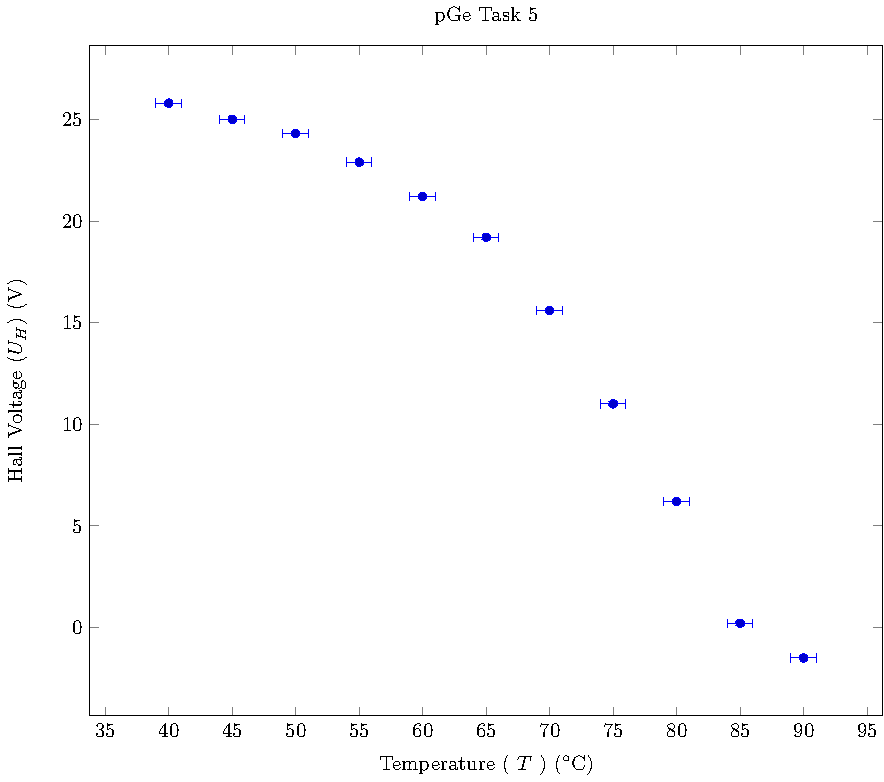
\includegraphics[width=0.7\textwidth]{PGePlots/Task5/pGeTask5.pdf}
\captionof{figure}{Hall voltage is plotted as a function of temperature.}
\label{task25plot}
\end{figure}

% Comment on the nature of the graph and different regions
% Discuss shape expected by theory

\subsubsection{Conclusion}
%Brief summary, discussion of results and theory
\qq This task was a success! The plot in Figure \ref{task25plot} clearly shows
the Germanium's shift from acting as an intrinsic conductor at lower
temperatures to acting as an extrinsic conductor at higher temperatures.

\section{Hall Effect in N-Germanium}

\subsection{Task 1}

\qq The dependence of the Hall voltage on the current was determined 
by modulating current and holding the magnetic field and temperature 
constant. Please note that the manual called for the magnetic field to 
be held at 250 mT, but it was instead kept at 144 mT in order to 
avoid reaching the maximum amperage on the coils. The corresponding
applied coil current was 4 A.

\subsubsection{Data Analysis and Results}
%Graphs, figures, and tables with captions
%Results with error analysis
%Calculate discrepancies from theory
%Discuss results and uncertainties
%Compare results with theory
\qq The Hall voltage and sample current maintain a linear
relationship, as seen in section 1.1, such that $U_H = \alpha *
I$. This is shown in figure \ref{task31plot}.

% Experimental data 
\begin{figure}[H]
\centering
% uncomment the line below to add image
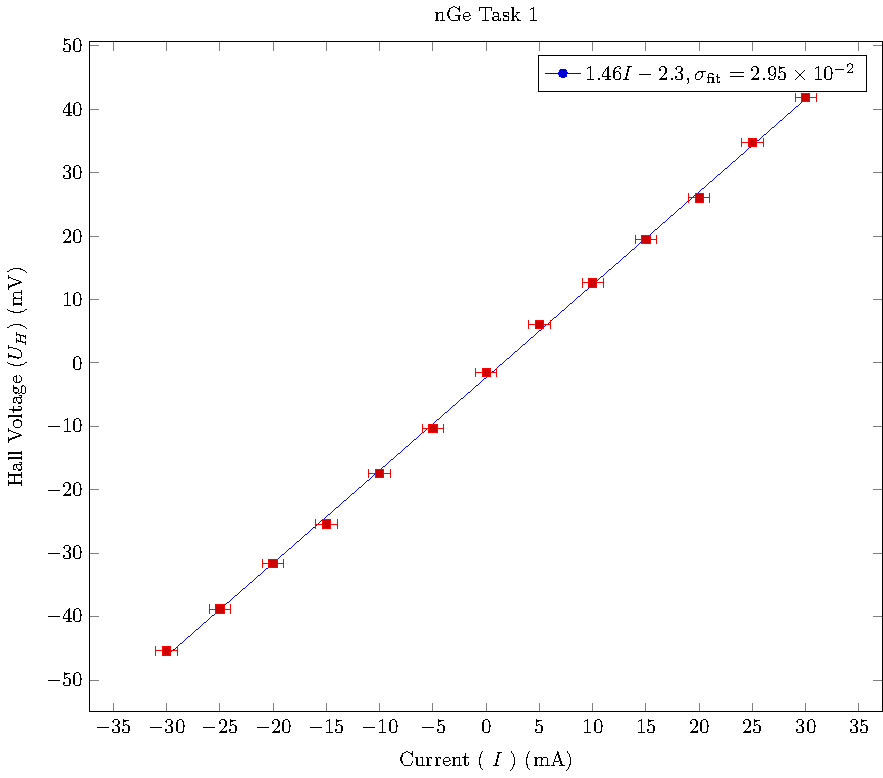
\includegraphics[width=0.7\textwidth]{NGePlots/Task1/nGeTask1.pdf}
\captionof{figure}{Hall voltage as a function of sample current 
in n-type Germanium. The linear fit has an $R^2$ value of 1.}
\label{task31plot}
\end{figure}

% Calculate theoretical proportionality constant
\qq Once again, a value for $\alpha_{theo}$ is determined from the
slope of the plot in figure \ref{task31plot}, where $B$ is the applied
magnetic field, $n$ is the density of charge carriers, $e$ is the
elementary charge, and $t$ is the sample thickness.
\begin{align*}
\alpha_{theo} &= \frac{B}{net} \\
              &= \frac{(0.144)}{(1.5 * 10^(21))*(1.6 * 10^(-19))*(1.0 * 10^(-3))} \\
			  &= 0.6 \\
\end{align*}

\subsubsection{Conclusion}
%Brief summary, discussion of results and theory
The experimental constant of proportionality $\alpha = 1.46 $ V/A is
within 2 $\sigma$ of the theoretical value $\alpha_{theo} = 0.6 $ V/A.

\subsection{Task 2}

\qq The dependence of the sample voltage on magnetic induction was
determined. The control current was held at a constant 30 mA. The
resistance was computed from the sample voltage and expressed as a
change in resistance relative to the resistance with no field.

\subsubsection{Data Analysis and Results}
%Graphs, figures, and tables with captions
%Results with error analysis
%Calculate discrepancies from theory
%Discuss results and uncertainties
%Compare results with theory
\qq Analysis was carried out in the same manner as the p-Germanium
experiment. The change is resistance was normalized against the
resistance with no applied field, and this was plotted against the
magnetic field strength, as shown in figure \ref{task32plot}.

% Experimental data 
\begin{figure}[H]
\centering
% uncomment the line below to add image
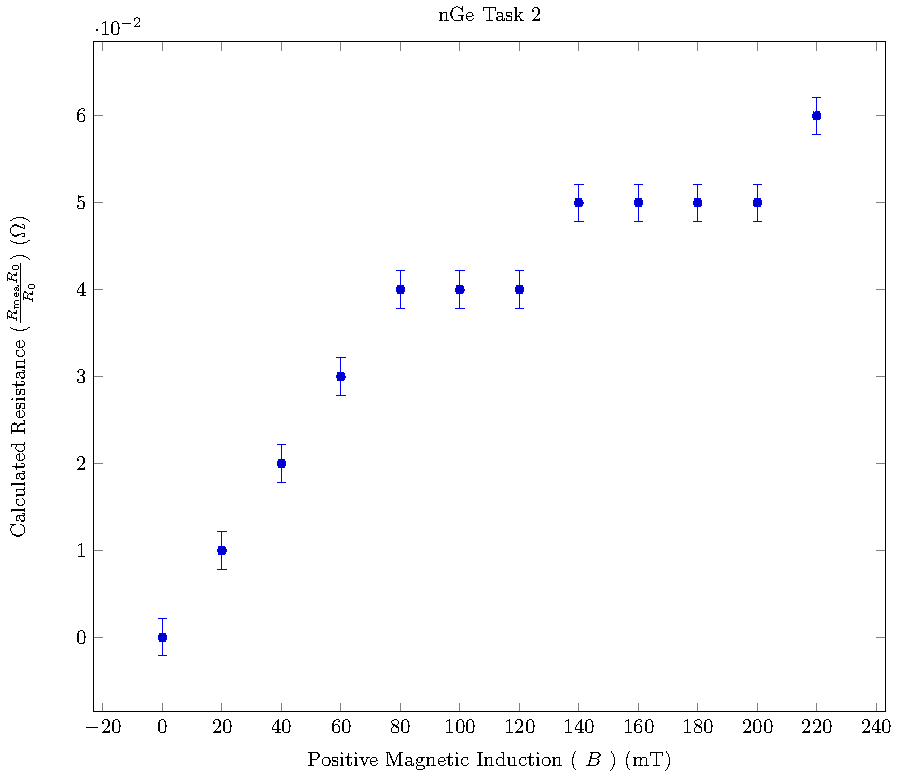
\includegraphics[width=0.7\textwidth]{NGePlots/Task2/nGeTask2.pdf}
\captionof{figure}{Normalized change in resistance against applied field strength.}
\label{task32plot}
\end{figure}


\subsubsection{Conclusion}
%Brief summary, discussion of results and theory
\qq There is a quadratic relationship between the normalized change in
resistance and the magnetic field strength.

\subsection{Task 3}
\qq A constant current of 30 mA is applied, and the sample voltage is
 measured as a function of temperature. The magnetic field remains off
 for this task. Note the maximum temperature was again limited to
 $110^o$ C.

\subsubsection{Data Analysis and Results}
%Graphs, figures, and tables with captions
%Results with error analysis
%Calculate discrepancies from theory
%Discuss results and uncertainties
%Compare results with theory
\qq The reciprocal of the voltage was plotted against the reciprocal
of the temperature. The data, shown in figure \ref{task33plot}, is
represented by a quadratic function.

% Experimental data 
\begin{figure}[H]
\centering
% uncomment the line below to add image
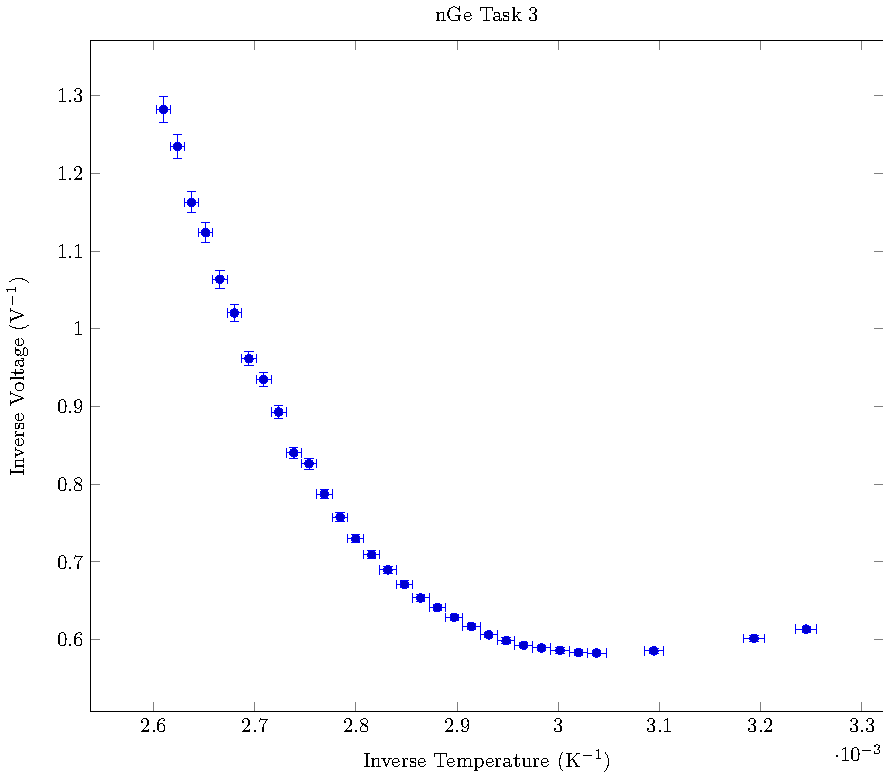
\includegraphics[width=0.7\textwidth]{NGePlots/Task3/nGeTask3Norm.pdf}
\captionof{figure}{Inverse voltage is plotted against inverse
  temperature for n-type Germanium.}
\label{task33plot}
\end{figure}

\qq The intrinsic conductivity is again approximated as the inverse
voltage, and the conductivity is related to the inverse temperature by
the relation $\sigma = \sigma_0 e^{-E_g/2kT}$. The natural logarithm
of conductivity is computed to produce the linear relation in figure
\ref{task33plotLINEAR}

% Calculated data 
\begin{figure}[H]
\centering
% uncomment the line below to add image
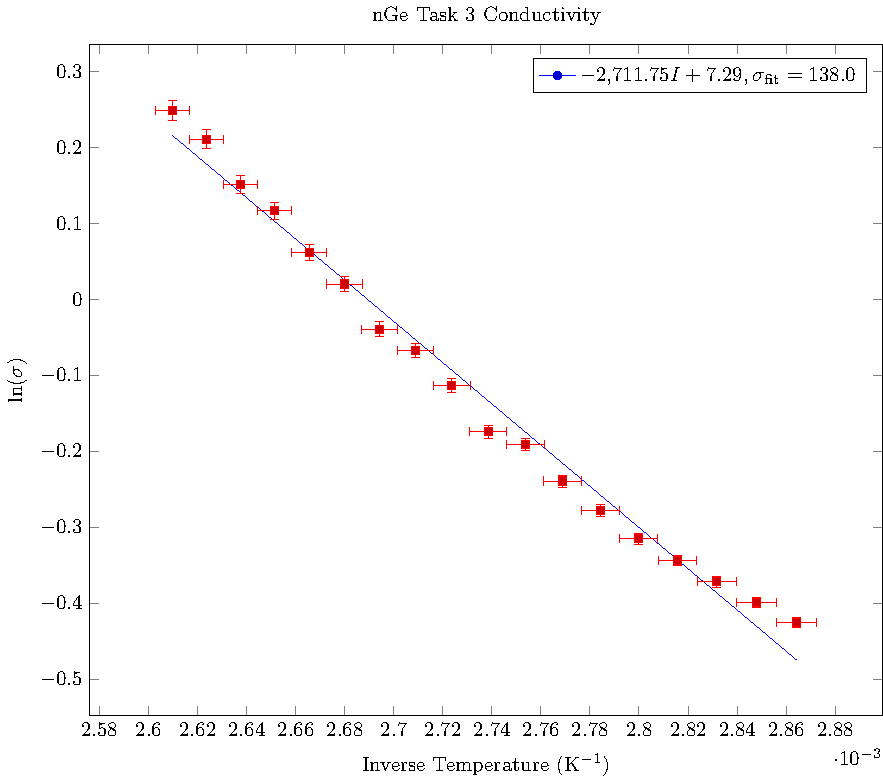
\includegraphics[width=0.7\textwidth]{NGePlots/Task3/nGeTask3Ln.pdf}
\captionof{figure}{Natural logarithm of conductivity versus inverse
  temperature for n-type Germanium}
\label{task33plotLINEAR}
\end{figure}

% Compute Eg experimentally
Again, an experimental value for the band gap energy is computed.
\begin{align*}
E_g &= - \text{SLOPE} \times 2k \\
    &= - (-3252) \times 2 
       \Big( (8.63 *10^(-5) \frac{eV}{K} \Big) \\
    &= 0.56 eV \\
\end{align*}

% Experimental error
The associated error in $E_{g_{exp}}$ can be computed from the error in the slope.
\begin{align*}
\delta_{Eg_{exp}} &= {138}*{2k} \\
                  &= {138}*{2*(8.63 *10^(-5))} \\
                  &= 0.024 eV \\
\end{align*}

% Difference and discrepancy
\qq The discrepancy is computed between the experimental and the
theoretical value band gap energy. The associated error is taken as
the error in the experimental value.
\begin{align*}
\delta_{E_g} &= | E_{g_{exp}} - E_{g_{theo}} | \\
		     &= | 0.56 - 0.50| \\
		     &= 0.06 eV \\
\end{align*}\\

\subsubsection{Conclusion}
%Brief summary, discussion of results and theory
\qq The experimental energy gap $E_{g_{exp}} = 0.56 eV$ is within
3 $\sigma$ of the theoretical value $E_{g_{theo}} = 0.50  eV$,
thus the values are in agreement.

\subsection{Task 4}

\qq The Hall voltage was measured as a function of the magnetic
induction, with constant temperature and current held at 30 mA. 
The field strength was limited to 290 mT. 

\subsubsection{Data Analysis and Results}
%Graphs, figures, and tables with captions
%Results with error analysis
%Calculate discrepancies from theory
%Discuss results and uncertainties
%Compare results with theory

% Calculated data 
\begin{figure}[H]
\centering
% uncomment the line below to add image
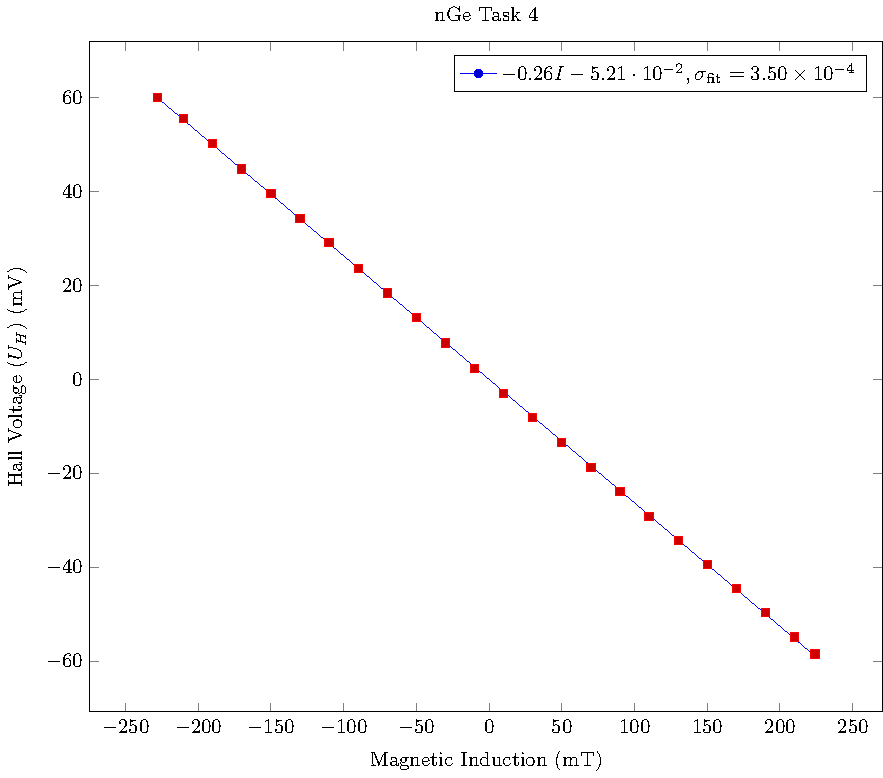
\includegraphics[width=0.7\textwidth]{NGePlots/Task4/nGeTask4.pdf}
\captionof{figure}{Hall voltage plotted as a function of applied
  magnetic field strength for n-type Germanium.}
\label{task34plot}
\end{figure}

% Experimental calculation of hall constant
\qq The experimental Hall constant is given by the slope, \( b =
\SI{0.26}{\volt\per\tesla} \), of Figure \ref{task34plot}
multiplied by \( \frac{d}{I} \), where \( d = \SI{1e-3}{\meter} \) is the
thickness of the sample and \( I = \SI{30}{\milli\ampere} \) is the applied
current. The calculation is carried 
out below.

\begin{align*}
  R_{\text{H}} &= b \frac{d}{I} \\
  R_{\text{H}} &= (0.65) \frac{(\num{1e-3})}{(\num{30e-3})} \\
  R_{\text{H}} &= \num{0.022}\si{\cubic\meter\per\ampere\per\second} \\
\end{align*}

% Error in experimental hall constant
\qq Since the only variable, the slope \( b \), is being multiplied by the constant
\( \frac{d}{I} = \num{0.0333} \), the error in the experimental hall constant is
merely the error in the slope, \( \delta b = \SI{3.5e-3}{\volt\per\tesla} \),
multiplied by the constant.

\begin{align*}
  \delta R_{\text{H}} &= \delta b \frac{d}{I} \\
  \delta R_{\text{H}} &= (\num{3.5e-3}) (\num{0.0333}) \\
  \delta R_{\text{H}} &= \SI{11.66e-5}{\cubic\meter\per\ampere\per\second} \\
\end{align*}

% Discrepancy compared to theory
\qq The theoretical value of the Hall constant is
\SI{4.8e-3}{\cubic\meter\per\ampere\per\second}. Therefore, the discrepancy
between our experimental value and this theoretical value is

\begin{align*}
  \Delta_{R_{\text{H}}} &= | R_{\text{H}_{\text{theo}}} - R_{\text{H}_{\text{exp}}} | \\
  \Delta_{R_{\text{H}}} &= | (\num{4.8e-3}) - (\num{8.66e-3}) | \\
  \Delta_{R_{\text{H}}} &= \SI{3.86e-3}{\cubic\meter\per\ampere\per\second} \\
\end{align*}


% Experimental calculation of carrier concentration
\qq The charge carrier concentration is calculated from the elementary
charge and experimental Hall constant.
\begin{align*}
n_{exp} &= \frac{1}{e \times R_{H_{exp}}} \\
	&= \frac{1}{(1.602 \times 10^{-19} As) \times (8.66 \times 10^{-3} 1/As)} \\
	&= 7.21 * 10^(20)
\end{align*}

% Experimental error
The associated error in $n_{exp}$ is calculated as follows.
\begin{align*}
\delta_n &= NEEEDDD \\
\end{align*}

% Theoretical carrier concentration
A similar calculation is performed with the theoretical Hall constant.
\begin{align*}
n_{theo} &= \frac{1}{e \times R_{H_{theo}}} \\
	&= \frac{1}{(1.602 * 10^(-19)) * (4.8 * 10^(-3))} \\
         &= 1.30*10^(21)
\end{align*}

% Discrepancy
The difference in experimental and theoretical Hall constant is calculated as follows.
\begin{align*}
\Delta &= | n_{exp}} - n_{theo}} | \\
       &= | 7.21* 10^(20) - 1.30*10^(21)|
       &= 5.79 * 10^(20)
\end{align*}

% SOURCES OF ERROR IN EXPERIMENT

\subsubsection{Conclusion}
%Brief summary, discussion of results and theory

\subsection{Task 5}

\subsubsection{Data Analysis and Results}
%Graphs, figures, and tables with captions
%Results with error analysis
%Calculate discrepancies from theory
%Discuss results and uncertainties

%Compare results with theory
% Discuss shape expected by theory                                                     
\qq The shape of the graph can be described by three differing
regions. The first relatively flat area in the region of the lower
temperatures depicts an extrinsic conduction. The middle section of
the graph that is described by the slope shows the reduction in the
drift velocity that is associated with the increase of charge carriers
with an increase of temperature. The third area, which is once again
relatively flat, described by the higher temperatures depicts the
intrinsic conduction. While the graph as a whole shows the transition
from extrinsic conduction to intrinsic conduction.

\begin{figure}[H]
  \begin{center}
    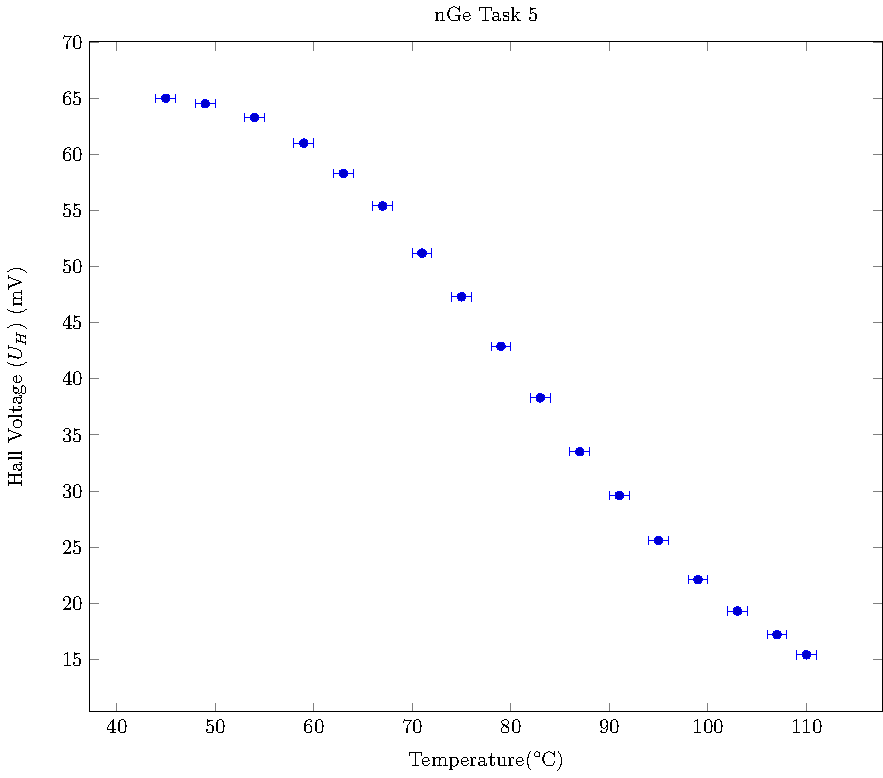
\includegraphics[scale=0.7]{NGePlots/Task5/nGeTask5.pdf}
  \end{center}
  \caption{The plot of Hall Voltage in millivolts versus temperature in Celsius
    showing the three regions.}
  \label{gph:nt5}
\end{figure}

\subsubsection{Conclusion}
\qq The plot in Figure (\ref{gph:nt5}) closely resembles what is expected. It
shows the three distinct trends in voltage as temperature increases.

\newpage

\section{Hall Effect in Pure Germanium}

\subsection{Determining Band Gap in Pure Ge}

\qq For semiconductors the conductivity is a function of
temperature. In this experiment, the current is held constant at 5 mA
and the induced magnetic field willl remain off. The sample voltage
was measured as a function of the temperature of the sample. The
conductivity can be approximated as the inverse voltage. The
conduc\ \ tivity is related to the inverse temperature by the relation
$\sigma = \sigma_0 e^{-E_g/2kT}$.This will allow one to create a graph
of the conductivity as a function of the inverse
temperature. Furthermore, plotting the natural logarithmic of the
conductivity versus the inverse temperature will result in a linear
plot. Using the slope of this plot the energy band gap is then
determined.

\subsubsection{Data Analysis and Results}
%Graphs, figures, and tables with captions
\qq To calculate the energy band gap the following equation can be
used, please note that 'k' represents the Boltzmann constant.

\begin{figure}[H]
  \begin{center}
    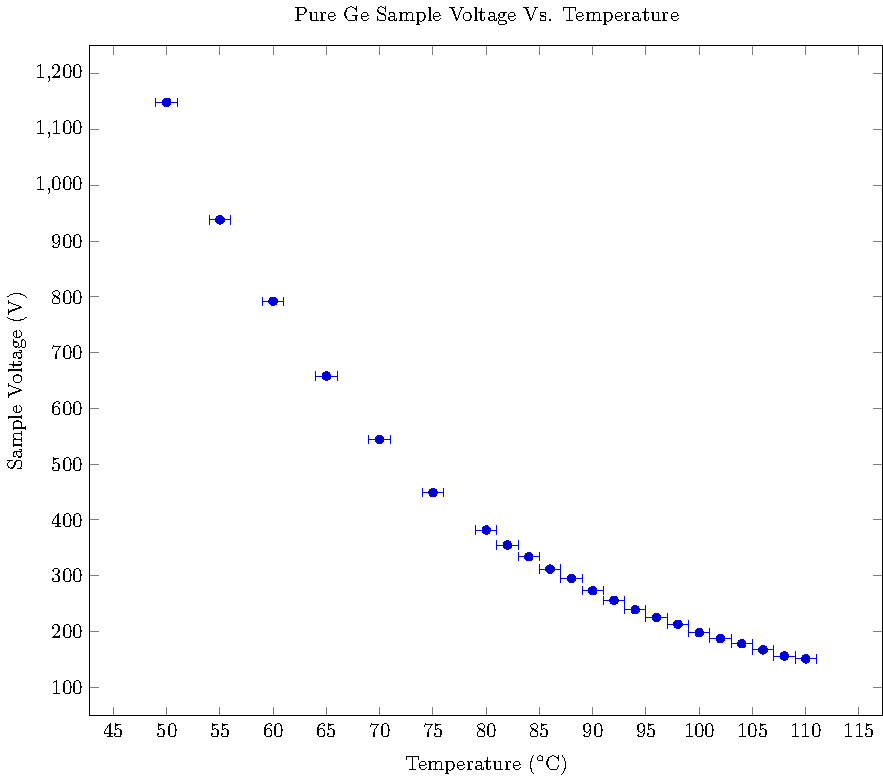
\includegraphics[scale=0.7]{PureGePlots/pureGeSamVoltVsTemp.pdf}
  \end{center}
  \caption{The plot of the voltage across the sample as its temperature changed.}
\end{figure}

\begin{figure}[H]
  \begin{center}
    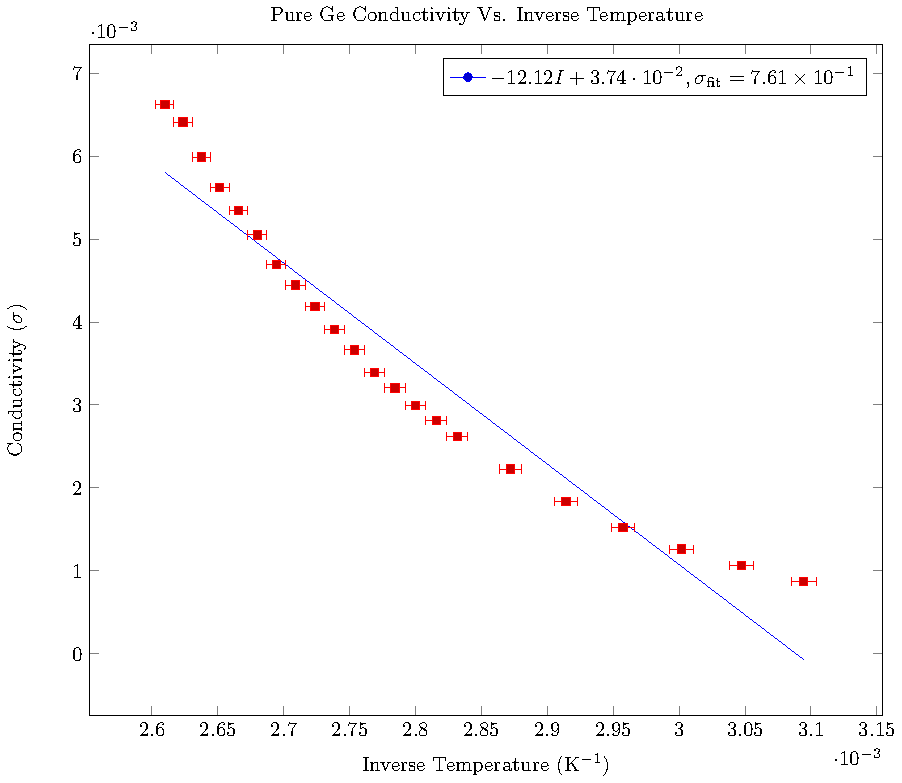
\includegraphics[scale=0.7]{PureGePlots/pureGeCondVsInvTemp.pdf}
  \end{center}
  \caption{The plot of the conductivity versus the inverse temperature.}
\end{figure}

% Compute Eg experimentally                              
\begin{align*}
E_g &= - \text{slope} \times 2k \\
    &= - (-4187) \times 2
       \Big(( 8.625 * 10^(-5)) \frac{eV}{K} \Big) \\
    &= 0.72 eV \\
\end{align*}

% Experimental error                                                                    
The associated error in $E_{g_{exp}}$ can be computed from the error in the slope.
\begin{align*}
\delta_{Eg_{exp}} &= {(7.21*10^(-1))*2*k} \\
                  &= (7.21*10^(-1))*(2)*(8.63*10^(-5))
                  &= 1.24*10^(-4)
\end{align*}

% Difference and discrepancy                                                                                   
\qq The discrepancy is computed between the experimental and the
theoretical value band gap energy. The associated error is taken as
the error in the experimental value.
\begin{align*}
\delta_{E_g} &= | E_{g_{exp}} - E_{g_{theo}} | \\
                     &= | 0.72 - 0.67| \\
                     &= 0.05 eV \\
\end{align*}\\

\subsubsection{Conclusion}
%Brief summary, discussion of results and theory                                                               
\qq The experimental energy gap $E_{g_{exp}} = 0.72 eV$ is within
1 $\sigma$ of the theoretical value $E_{g_{theo}} = 0.67  eV$,
thus the values are in agreement.


\section{Hall Effect in Pure Zinc}

\subsection{Determining Hall Constant in Pure Zn}

\subsubsection{Data Analysis and Results}
%Graphs, figures, and tables with captions
%Results with error analysis
%Calculate discrepancies from theory
%Discuss results and uncertainties
%Compare results with theory
\qq In order to determine the Hall constant $\text{R}_\text{H}$, one can
analyze the dependence of the Hall voltage on the applied field. This
was done with a constant DC current applied across the Zinc sample, with
an associated random error due to the limited precision of the power
supply. The error in the slope is obtained through linear regression,
and the thickness prescribed by the sample specifications is assumed
to have no error.

\begin{center}
\begin{tabular}{|c|c|}
\hline Slope, $b$ $\big[ \frac{\Omega \text{cm}}{\text{G}} \big] $ &
$4.11 \times 10^{-13} \pm ERROR$ \topVspace \bottomVspace \\ \hline
Thickness, $d$ [m] & $2.5 \times 10^{-5} \pm
0$ \topVspace \bottomVspace \\ \hline Sample Current, I [A] & $13.5
\pm 0.1$ \topVspace \bottomVspace \\ \hline
\end{tabular}
\label{table:zinc_RH}
\captionof{table}{Measurements and calculations used to determine the
  experimental Hall constant of pure Zinc}
\end{center}

\begin{figure}[H]
  \begin{center}
    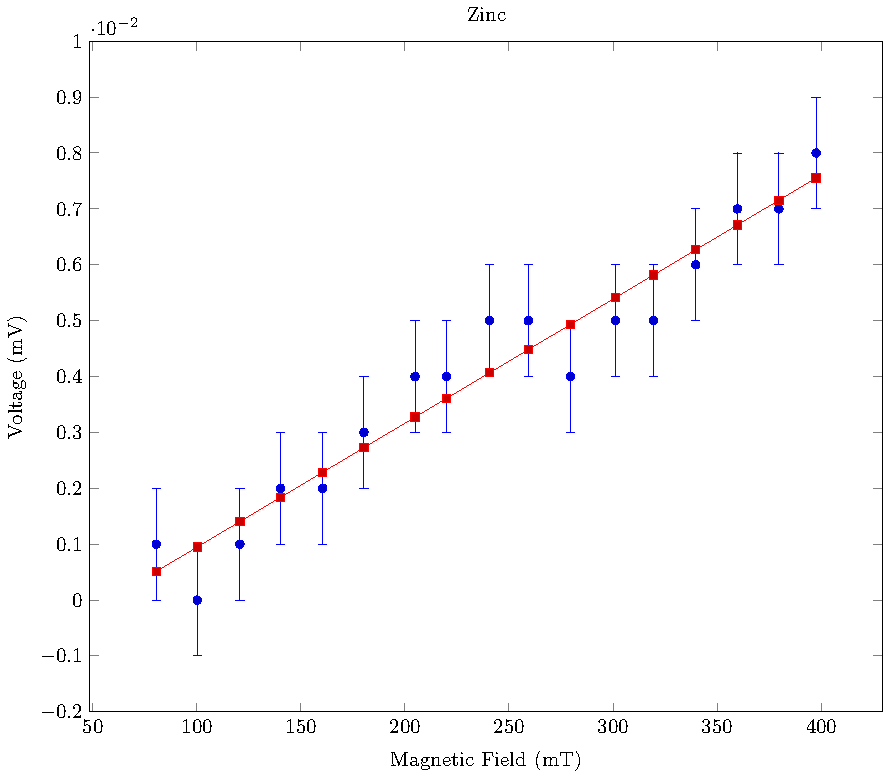
\includegraphics[scale=0.7]{ZincPlot/zincPlot.pdf}
  \end{center}
\end{figure}

% Finding experimental hall constant
The Hall constant of Zinc is calculated as follows.
\begin{align*}
R_{H_{exp}} &= \big( \frac{\mu_H}{B} \big) \, \frac{d}{I} \\
    &= (b) \, \frac{d}{I} \\
    &= (4.11 \times 10^{-13}) \, \frac{2.5 \times 10^{-5}}{13.5} \\
    &= 4.11 \times 10^{-11} \; \text{Vm/TA} \\
    &\equiv 4.11 \times 10^{-13} \; \Omega \text{cm/G} \\
\end{align*}

% Finding experimental aerror
The uncertainty in the experimental Hall constant is propagated as follows.
\begin{align*}
\delta R_{H_{exp}} &= | R_{H_{exp}} | 
                      \sqrt{
                      	\Big( \frac{\delta b}{b} \Big) ^2
                      	+
                      	\Big( \frac{\delta d}{d} \Big) ^2
                      	+
                      	\Big( \frac{\delta I}{I} \Big) ^2
                      } \\
                       &=
                   	 \sqrt{
                      	\Big( \frac{SLOPERROR}{4.11 \times 10^{-13}} \Big) ^2
                      	+
                      	\Big( \frac{0}{2.5 \times 10^{-5}} \Big) ^2
                      	+
                      	\Big( \frac{0.1}{13.5} \Big) ^2
                      } 
\end{align*}

% Getting theoretical hall constant and error
\qq A theoretical value for the Hall constant of Zinc, given by the
third edition of the AIP handbook, is $R_H = 3.30 \times 10^{-13} \;
\Omega \text{cm/G}$. This theoretical Hall constant has no given
associated error, so the associated discrepancy, $\Delta$, will simply
equal that of the experimental Hall constant. The following
computations are thus performed.

% Finding discrepancy
\begin{align*}
\Delta &= | R_{H_{exp}} - R_{H_{theo}} | \\
	   &= | (4.11 \times 10^{-13}) - (3.30 \times 10^{-13}) | \\
\end{align*}

% Finding error in discrepancy
\begin{align*}
\delta_{\Delta} &= \delta R_{H_{exp}} \\
				&= \text{COPY VALUE FROM ABOVE} \\
\end{align*}

\subsubsection{Conclusion}
%Brief summary, discussion of results and theory
\qq It is evident that the discrepancy is within SOMENUMBER $\sigma$,
so the experimental Hall constant $R_{H_{exp}} = 4.11 \times 10^{-13}
\Omega \text{cm/G}$ (AGREES / DOES NOT AGREE) with the reported
theoretical value $R_{H_{theo}} = 3.30 \times 10^{-13} \Omega
\text{cm/G}$.

\section{Sources of Error}
\qq Some sources of error can be found in this experiment. One such
source is that the coils produce a latent magnetic field when they are
turned off, which is a systematic error. There is also a systematic
error due to the thermal energy loss during the tasks that are
dependent on temperature. Some random errors occured due to the
equipment. One such error was the multimeter which varried our results
when the was movement around the meter. Another such error was the
power supply did not keep a steady AC current.

\section{Appendices}

\subsection{Appendix A: Data}

\subsection{Appendix B: Source Code}

\end{document}
